\documentclass[tikz]{standalone}

\usepackage{amsmath, amssymb}

\begin{document}
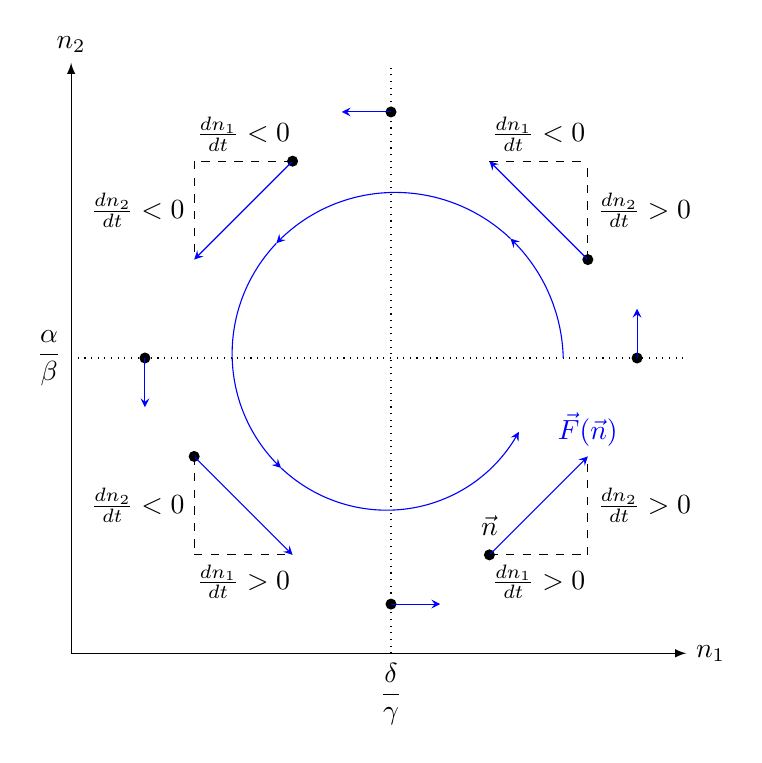
\begin{tikzpicture}[scale=1.25]
  \draw[-latex] (-0.25,0)--(6,0) node[right] {\(n_1\)};
  \draw[-latex] (-0.25,0)--(-0.25,6) node[above] {\(n_2\)};
  \draw[dotted] (3,0)--(3,6);
  \node[below] at (3,0) {\(\dfrac{\delta}{\gamma}\)};
  \draw[dotted] (-0.25,3)--(6,3);
  \node[left] at (-0.25,3) {\(\dfrac{\alpha}{\beta}\)};
                        %
  \filldraw (4,1) circle (0.05cm);
  \node[above] at (4,1.1) {\(\vec{n}\)};
  \draw[->,>=stealth,blue] (4,1)--(5,2) node[above] {\(\vec{F}(\vec{n})\)};
  \draw[dashed] (4,1)--(5,1);
  \node[below] at (4.5,1) {\(\frac{dn_1}{dt} >0\)};
  \draw[dashed] (5,1)--(5,2);
  \node[right] at (5,1.5) {\(\frac{dn_2}{dt}>0\)};
                        %
  \filldraw (5,4) circle (0.05cm);
  \draw[->,>=stealth,blue] (5,4)--(4,5);
  \draw[dashed] (4,5)--(5,5);
  \node[above] at (4.5,5) {\(\frac{dn_1}{dt} <0\)};
  \draw[dashed] (5,4)--(5,5);
  \node[right] at (5,4.5) {\(\frac{dn_2}{dt} >0\)};
                        %
  \filldraw (2,5) circle (0.05cm);
  \draw[->,>=stealth,blue] (2,5)--(1,4);
  \draw[dashed] (2,5)--(1,5);
  \node[above] at (1.5,5) {\(\frac{dn_1}{dt} <0\)};
  \draw[dashed] (1,5)--(1,4);
  \node[left] at (1,4.5) {\(\frac{dn_2}{dt} <0\)};
                        %
  \filldraw (1,2) circle (0.05cm);
  \draw[->,>=stealth,blue] (1,2)--(2,1);
  \draw[dashed] (1,1)--(2,1);
  \node[below] at (1.5,1) {\(\frac{dn_1}{dt} >0\)};
  \draw[dashed] (1,2)--(1,1);
  \node[left] at (1,1.5) {\(\frac{dn_2}{dt} <0\)};
                        %
  \filldraw (3,0.5) circle (0.05cm);
  \draw[->,>=stealth,blue] (3,0.5)--(3.5,0.5);
                        %
  \filldraw (5.5,3) circle (0.05cm);
  \draw[->,>=stealth,blue] (5.5,3)--(5.5,3.5);
                        %
  \filldraw (3,5.5) circle (0.05cm);
  \draw[->,>=stealth,blue] (3,5.5)--(2.5,5.5);
                        %
  \filldraw (0.5,3) circle (0.05cm);
  \draw[->,>=stealth,blue] (0.5,3)--(0.5,2.5);
                        %
  \draw[domain=0:45,samples=100,blue,->,>=stealth]
  plot( {3+(1.75 - 0.25*\x/330)*cos(\x) }, { 3+(1.75-0.25*\x/330)*sin(\x) } );
  \draw[domain=45:135,samples=100,blue,->,>=stealth]
  plot( {3+(1.75 - 0.25*\x/330)*cos(\x) }, { 3+(1.75-0.25*\x/330)*sin(\x) } );
  \draw[domain=135:225,samples=100,blue,->,>=stealth]
  plot( {3+(1.75 - 0.25*\x/330)*cos(\x) }, { 3+(1.75-0.25*\x/330)*sin(\x) } );
  \draw[domain=225:330,samples=100,blue,->,>=stealth]
  plot( {3+(1.75 - 0.25*\x/330)*cos(\x) }, { 3+(1.75-0.25*\x/330)*sin(\x) } );
\end{tikzpicture}
\end{document}
